\documentclass[a4paper,12pt]{article}
\usepackage[utf8]{inputenc}
\usepackage[T1]{fontenc}
\usepackage[french]{babel}
\usepackage{geometry}
\usepackage{amsmath}
\usepackage{amsfonts}
\usepackage{amssymb}
\usepackage{hyperref}
\usepackage{graphicx}
\usepackage{fancyhdr}
\geometry{margin=2.5cm}

\title{Expérience Professionnelle}
\author{Mignard Maël}
\date{\today}

\begin{document}

\maketitle
\section{Droits et Devoirs}

\vspace{1cm}
\subsection*{Le contrat d'apprentissage (CERFA)}
\begin{itemize}
    \item Contrat de travail conclu entre l'apprenti et l'employeur pour une période donnée (durée de la préparation du diplôme).
    \item Le contrat de travail doit respecter le Code du travail et, le cas échéant, la convention collective.
    \item Le temp passé a l'école est considéré comme du temps de travail effectif.
    \item La période d'essais est de 45 jours effectifs en entreprise.
\end{itemize}
\subsection*{Conditions de travail}
\begin{itemize}
    \item L'apprenti bénéficie des mêmes conditions de travail que les autres salariés de l'entreprise.
    \item Il acquiert 2 jours et demi de congés payés par mois de travail effectif.
    \item Il est interdit de poser des congés pendant les temps de formation.
    \item \textbf{Heures supplémentaires (interdites pour les alternants) :}
    \begin{itemize}
        \setlength\itemsep{0.3em}
        \item Maximum \textbf{10 heures par jour}.
        \item Maximum \textbf{48 heures par semaine}.
    \end{itemize}
\end{itemize}
\clearpage
\subsection{Exercice TD}
\vspace{1cm}
\textbf{consignes}
Comparatif entre droit du travail et Convention collective
\begin{itemize}
    \item Remuneration
    \item Congés payés
    \item Temps de travail
\end{itemize}
\vspace{1cm}
\subsubsection*{Travail de groupe}
\begin{figure}[h!]
    \centering
    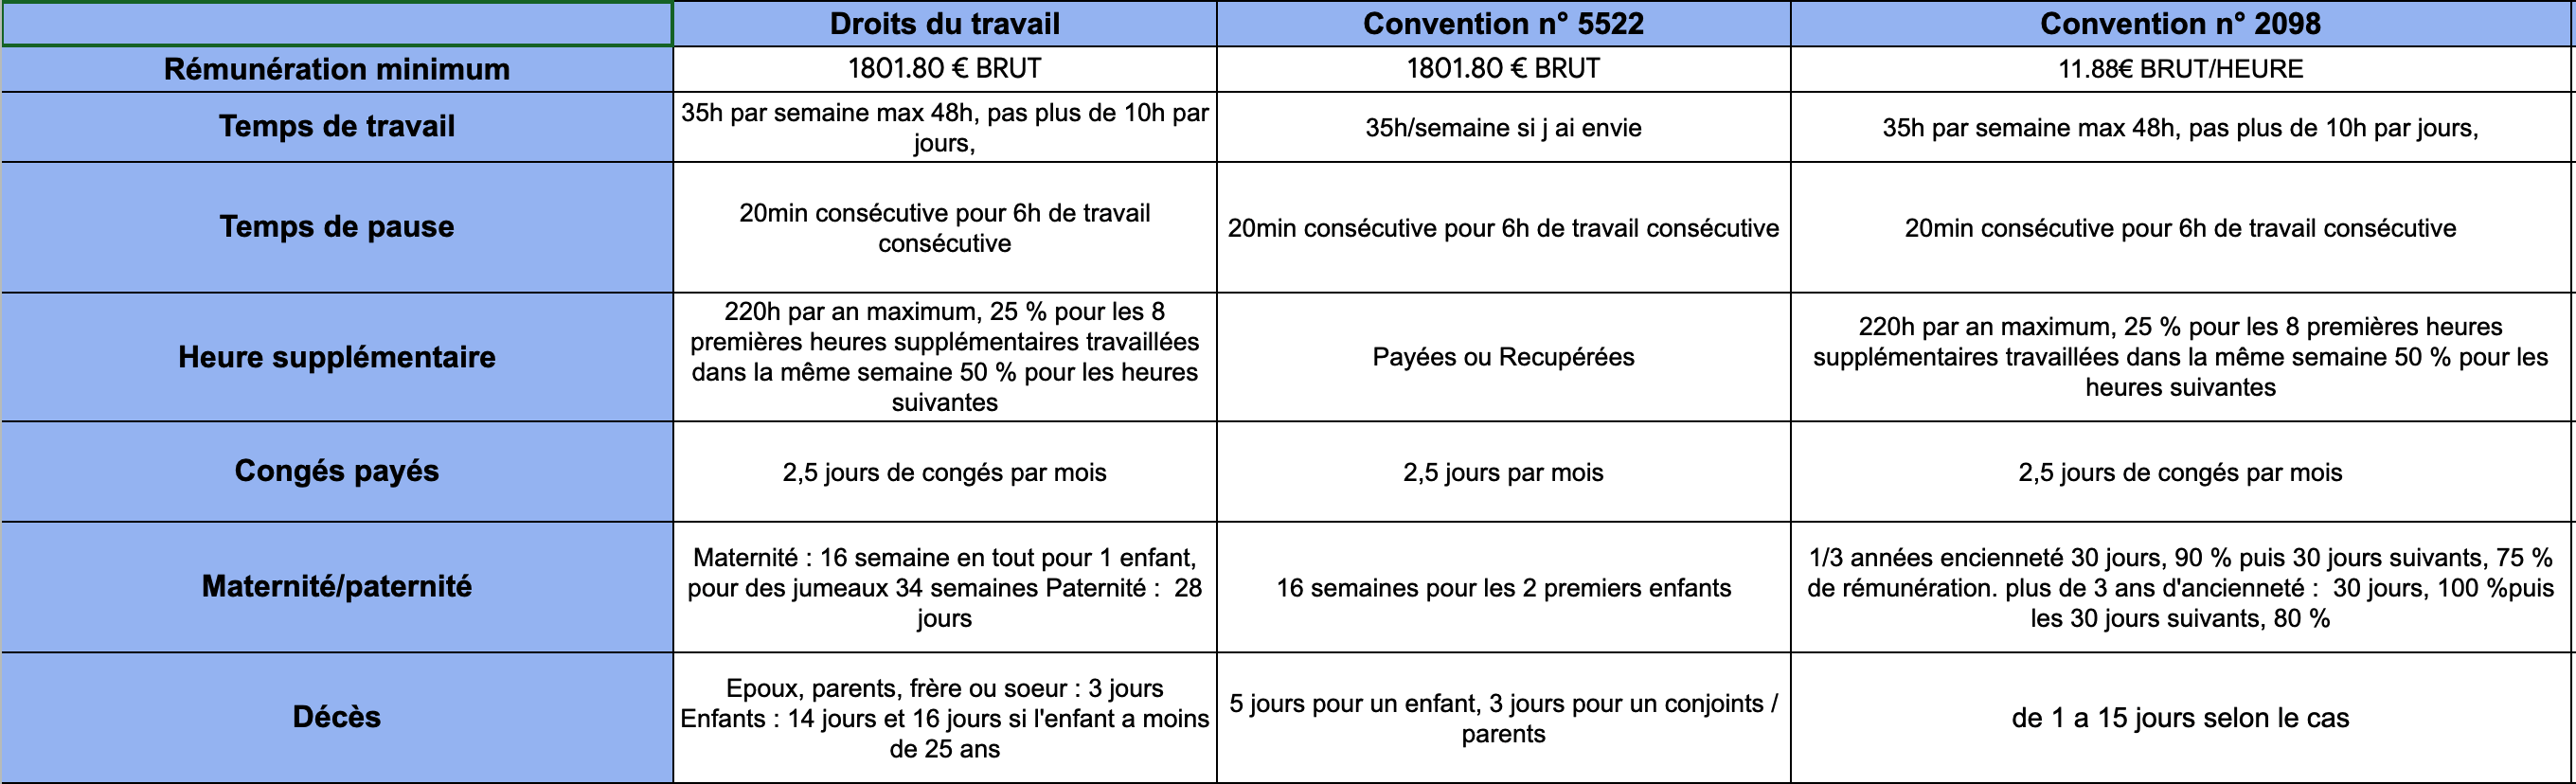
\includegraphics[width=0.8\textwidth]{Tableau Comparatif.png}
    \caption{Tableau Comparatif Droit du travail / Cocnventions Collectives}
    \label{fig:capture1}
\end{figure}
\end{document}
